\documentclass{article} % say 
\usepackage[paperheight=2048px,paperwidth=2048px,left=-15px,right=-10px,top=0px,bottom=0px,showframe]{geometry}
\usepackage{tikz}
\usetikzlibrary{backgrounds}
\begin{document}

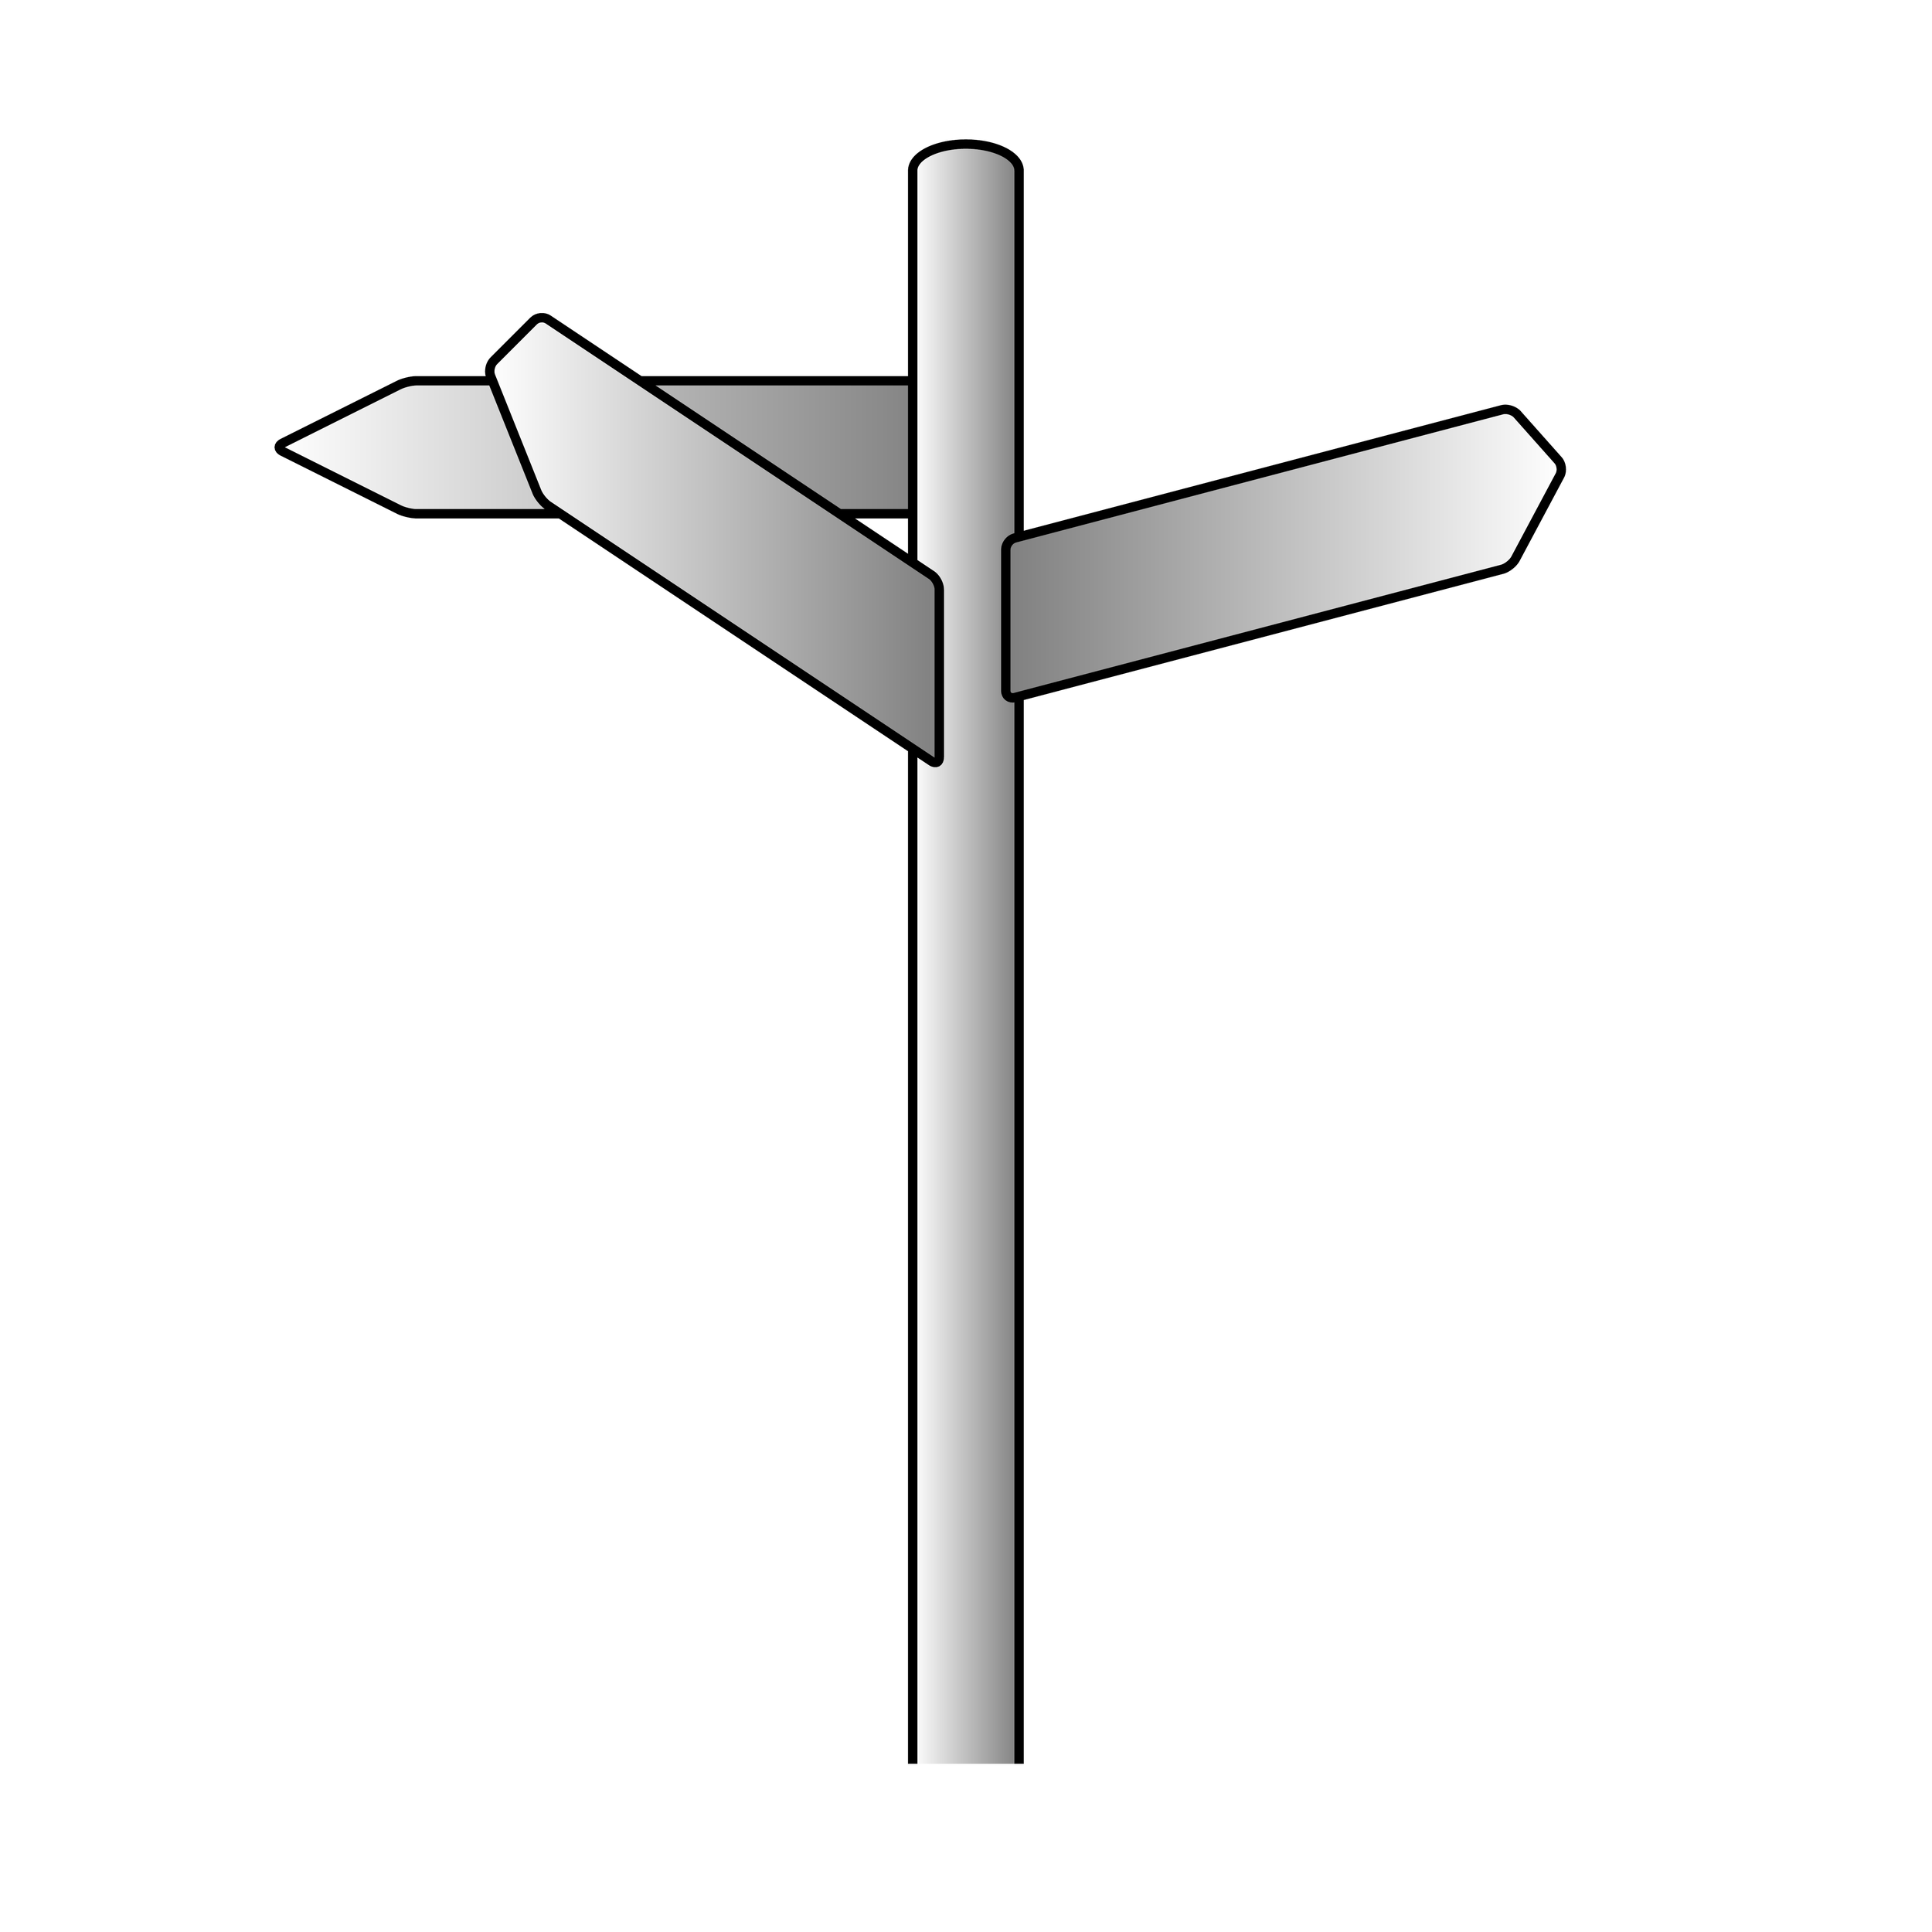
\begin{tikzpicture}[background rectangle/.style= {bottom color=white,top color=white,rounded corners}, show background rectangle]
  \clip (0,0) circle (35.9662);
  \shadedraw[left color=white,right color=black!50!white,line width=10pt,rounded corners=10pt] (-1,17) -- +(-20,0) -- +(-25,2.5) -- +(-20,5) -- +(0,5) -- cycle;
  \shadedraw[left color=white,right color=black!50!white,line width=10pt] (2,-30) -- (2,29.9) arc [start angle=0, end angle=180,x radius=2, y radius=1] -- (-2,-30);
  \shadedraw[left color=white,right color=black!50!white,line width=10pt,rounded corners=10pt] (-1,7.5) -- +(-15,10) -- +(-17,15) -- +(-15,17) -- +(0,7) -- cycle;
  \shadedraw[left color=black!50!white,right color=white,line width=10pt,rounded corners=10pt] (1.5,10) -- +(19,5) -- +(21,8.75) -- +(19,11) -- +(0,6) -- cycle;

\end{tikzpicture}

\end{document}
